\documentclass[c]{beamer}
\usepackage[utf8]{inputenc}
\usepackage[french]{babel}
\usepackage[T1]{fontenc}
\usepackage{amsmath,amssymb}
\usepackage{graphicx} 
\usepackage{wrapfig}
\usepackage{enumerate}
\usepackage{array} 
\usepackage{booktabs}
\usepackage{amsmath}
\usepackage{eso-pic}
\usepackage{animate}
\usepackage{multicol}
\usepackage{placeins}
\usepackage{xcolor}


\graphicspath{ {images/} }
\usetheme{Warsaw}
\setbeamertemplate{footline}
{
  \leavevmode%
  \hbox{%
  \begin{beamercolorbox}[wd=.5\paperwidth,ht=2.25ex,dp=1ex,center]{author in head/foot}%
    \usebeamerfont{author in head/foot}\insertshortauthor
  \end{beamercolorbox}%
  \begin{beamercolorbox}[wd=.35\paperwidth,ht=2.25ex,dp=1ex,center]{title in head/foot}%
    \usebeamerfont{title in head/foot}\insertshorttitle
  \end{beamercolorbox}%
  \begin{beamercolorbox}[wd=.15\paperwidth,ht=2.25ex,dp=1ex,right]{date in head/foot}%
    \usebeamerfont{date in head/foot}\hspace*{2em}
    \insertframenumber{} / \inserttotalframenumber\hspace*{2ex} 
  \end{beamercolorbox}}%
  \vskip0pt%
}

\title{Linear Reward Inaction} 

\author[C. BASKEVITCH, T. BESSAC, J. DESQUAIRES, B. LIU]{Claire BASKEVITCH,Tristan BESSAC,\\Joseph DESQUAIRES, Bin LIU}
\institute{Paris Saclay}
\date{Février 2020}
\logo{
\includegraphics[height=0.45cm]{Images/logo.png}}

\AtBeginSection[]{
  \begin{frame}{Sommaire}
  \small \tableofcontents[currentsection, hideothersubsections]
  \end{frame} 
}

%\AtBeginSubsection[]{
%  \begin{frame}{Sommaire}
%  \small \tableofcontents[hideothersubsections, currentsubsection]
%  \end{frame} 
%}

\begin{document}

\begin{frame}
\titlepage
\end{frame}
\begin{frame}{Sommaire}
\tableofcontents[pausesections]
\end{frame}

\section{Introduction}
\begin{frame}{Le jeu}
Il s'agit d'un jeu de poker simplifié où les 2 joueurs tirent une carte entre 1 et 9 en même temps.
\begin{block}{Alice joue en première - 4 choix :}
\begin{itemize}
    \item Se coucher.
    \item Relancer de 1.
    \item Relancer de 2.
    \item Relancer de 4.
\end{itemize}
\end{block}
\begin{exampleblock}{Bob joue toujours en deuxième - 2 choix :}
 \begin{itemize}
        \item Suivre la mise de Alice.
        \item Se coucher.
    \end{itemize}
\end{exampleblock} 

\end{frame}

%%%%%%%%%%%%%%%%%%%%%%%%%%%%%%ù

\section{Linear Reward Inaction}
\subsection{Principe}
\begin{frame}{Principe}
\begin{itemize}
    \item Repose sur un \textbf{principe de récompense} lors d'une action positive.
    \item \textbf{Ne prends en compte ni la perte ni l'égalité}.\\~\
    \item On a un \textbf{vecteur stochastique de stratégie} pour chaque carte et joueur qui \textbf{se met à jour uniquement lors d'un gain}.
    \item Permet de trouver un \textbf{équilibre de Nash (en stratégies pures)} pour un.
\end{itemize}
\end{frame}

\begin{frame}{Algorithme de LRI}
\begin{figure}
    \centering
    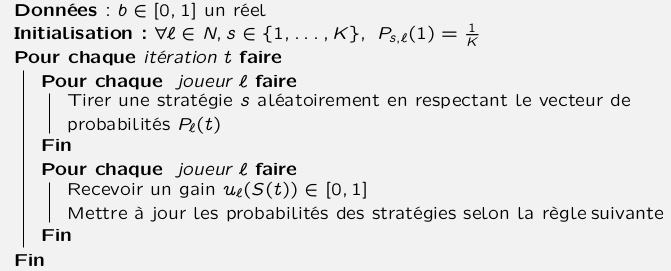
\includegraphics[width=\textwidth]{Images/algo/13.png}
    \label{fig:my_label}
\end{figure}
\centering K : nombre de stratégies.


%\begin{block}{Convergence de LRI [Sastry et Al. 1994]}
%\centering
%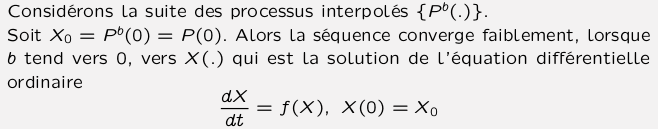
\includegraphics[width=0.60
%\textwidth,height=0.18\textheight]{Images/algo/14.png}
%\end{block}
\end{frame}

%%%%%%%
\begin{frame}{Mise à jour des stratégies des joueurs}
    \begin{block}{Règle de Mise à jour}
    $q_{i,s}(t+1)= \left\{\begin{array}{ll}
        q_{i,s}(t) + b * U_{t} * (1 - q_{i,s}(t))& \mbox{Si } s = s_i(t) \\
         q_{i,s}(t) - b * U_{t} * q_{i,s}(t) & \mbox{Si } s \neq s_i(t)
    \end{array}
\right.$
    \end{block}
    \begin{exampleblock}{Variables et constantes}
    \begin{description}
    \item[b] : paramètre d'apprentissage tq $b \in [0,1]$ et $b\leq \frac{1}{U_{max}}$.
    \item[$q_{i,s}(t)$] : probabilité que le joueur i joue la stratégie s à l'étape t.
    \item[$U_t$] : fonction d'utilité. %$U_t = \frac{Gain}{GainMax} =  \frac{Gain}{5}$
    \end{description}
    \end{exampleblock}
\end{frame}

%\begin{frame}{Propriété de la dynamique de LRI (Folk Theorem)}
%\begin{itemize}
%    \item Tous les équilibres de Nash sont des points stationnaires.
%    \item Tous les équilibres de Nash strict (en
%stratégies pures) sont asymptotiquement stables.
%    \item Tous les points stationnaires qui ne sont pas des Nash purs ne sont pas stables.
%\end{itemize}
%\end{frame}

\subsection{Application}

\begin{frame}{Étude de courbes}
\begin{columns}
        \begin{column}{0.5 \textwidth}
        \begin{small}
       \hspace{-0.24 cm} Probabilité qu'\textcolor{red}{Alice} se couche \\ Probabilité que \textcolor{blue}{Bob} se couche\\
        \end{small}
        \centering
            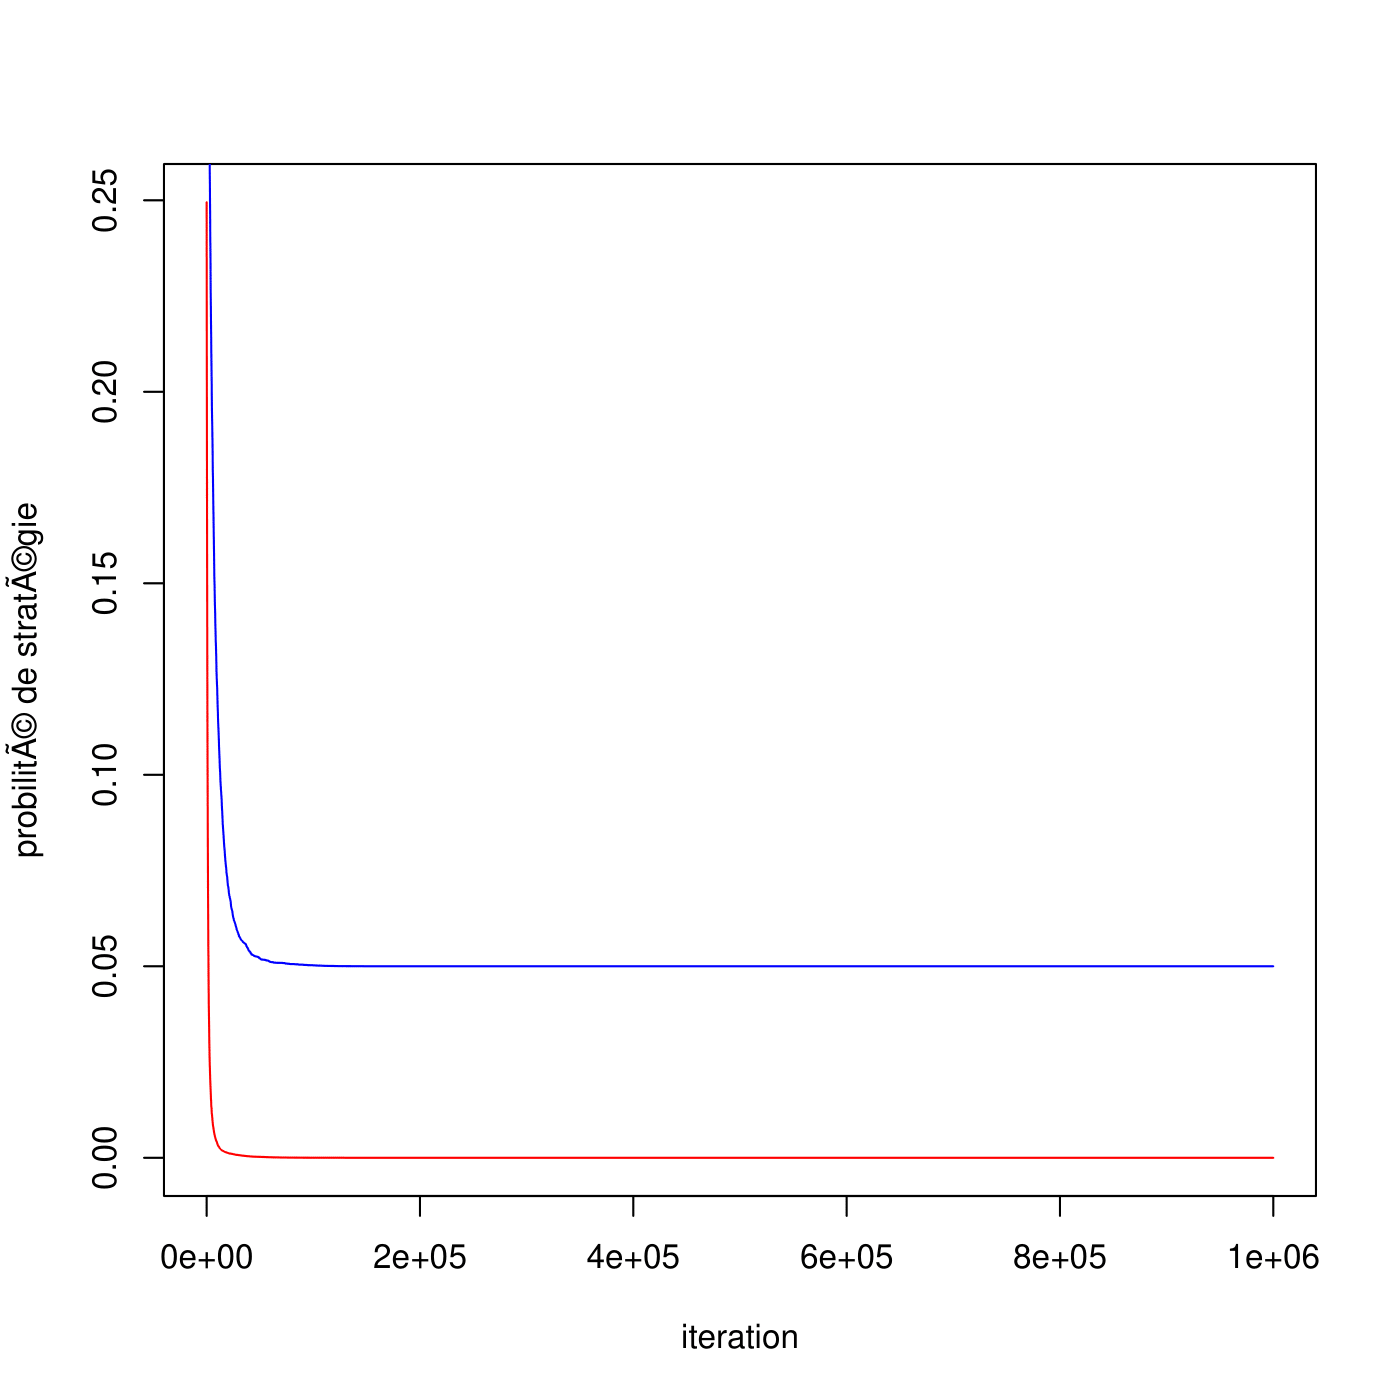
\includegraphics[width =\textwidth]{Images/Courbes/LRI/SeCoucher.png}
       
    
        \end{column}
       
        \begin{column}{0.5 \textwidth}
         \begin{small}
         \hspace{-0.24 cm} Probabilité qu'\textcolor{red}{Alice} relance de 4\\ Probabilité que \textcolor{blue}{Bob} suive\\
          \end{small}
        \centering
            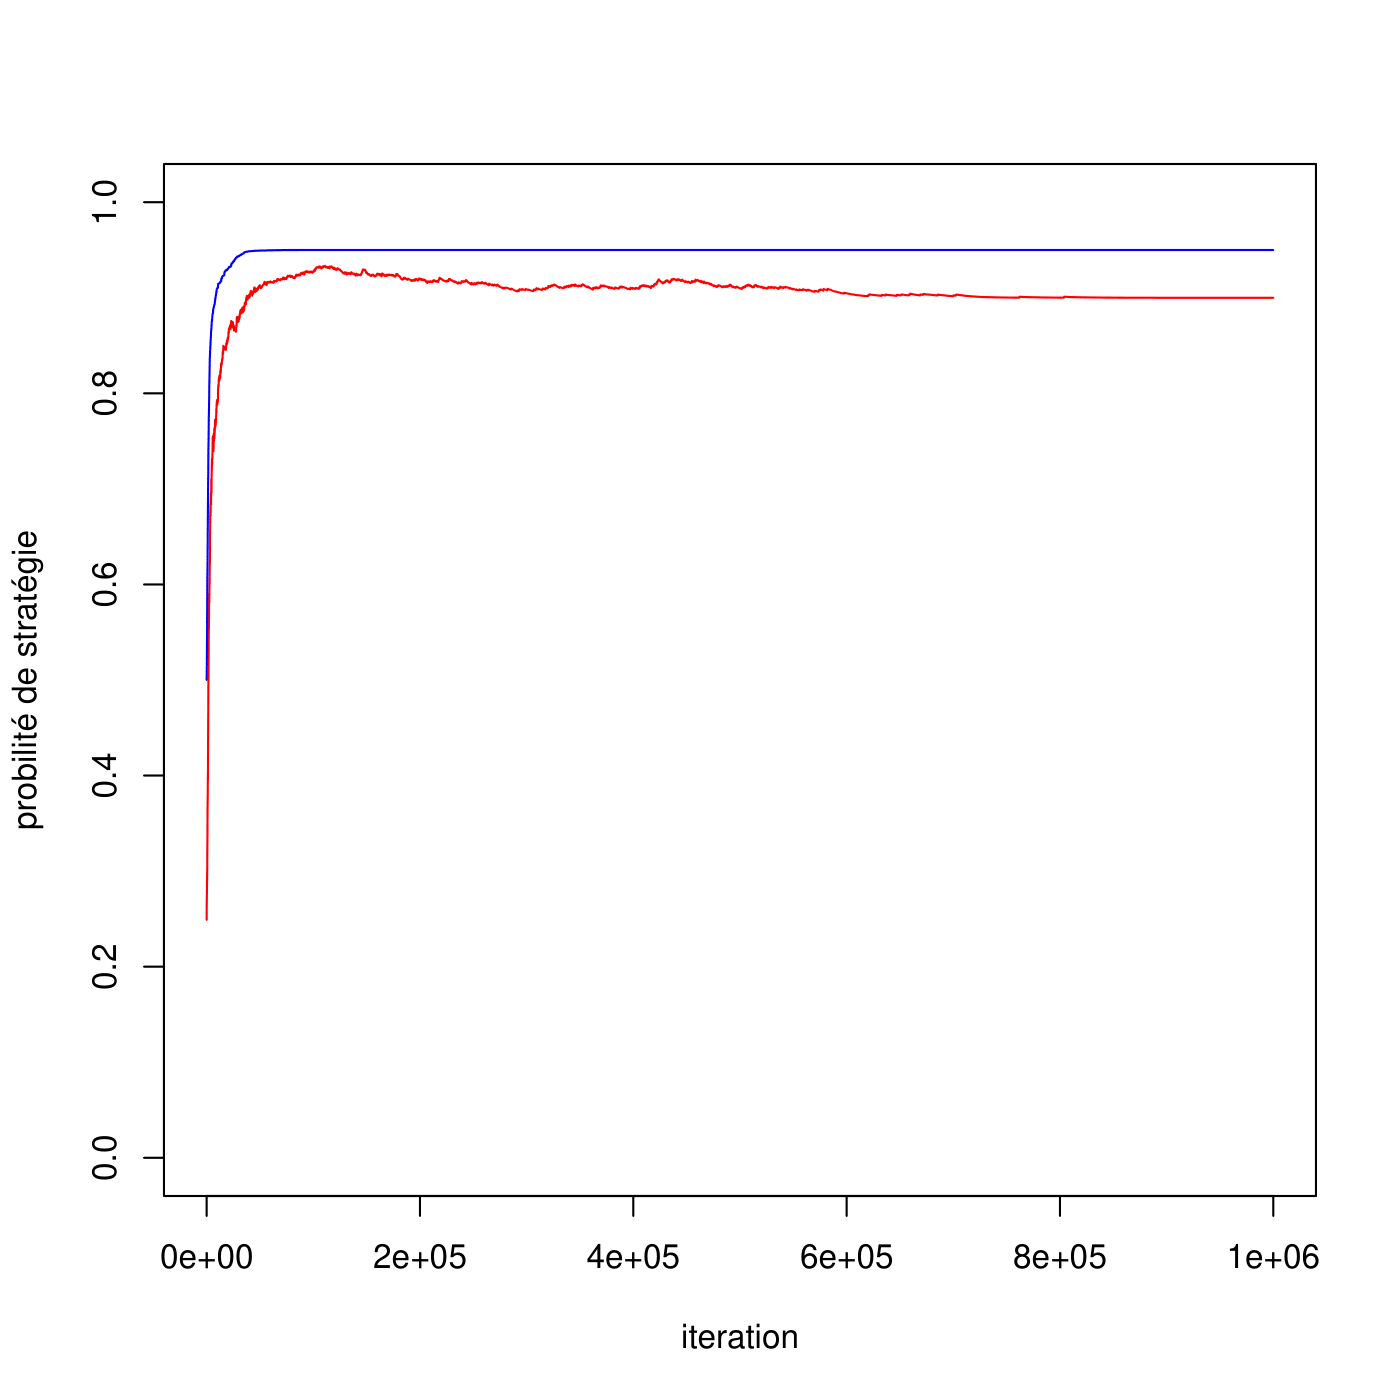
\includegraphics[width =\textwidth]{Images/Courbes/LRI/Relance4.png}
       
    \end{column}
    \end{columns}
\end{frame}

\begin{frame}{Étude de courbes}
\begin{columns}
        \begin{column}{0.5 \textwidth}
        \begin{small}
        \hspace{-0.24 cm} Probabilité qu'\textcolor{red}{Alice} relance de 1 \\ Probabilité que \textcolor{blue}{Bob} suive\\
        \end{small}
        \centering
            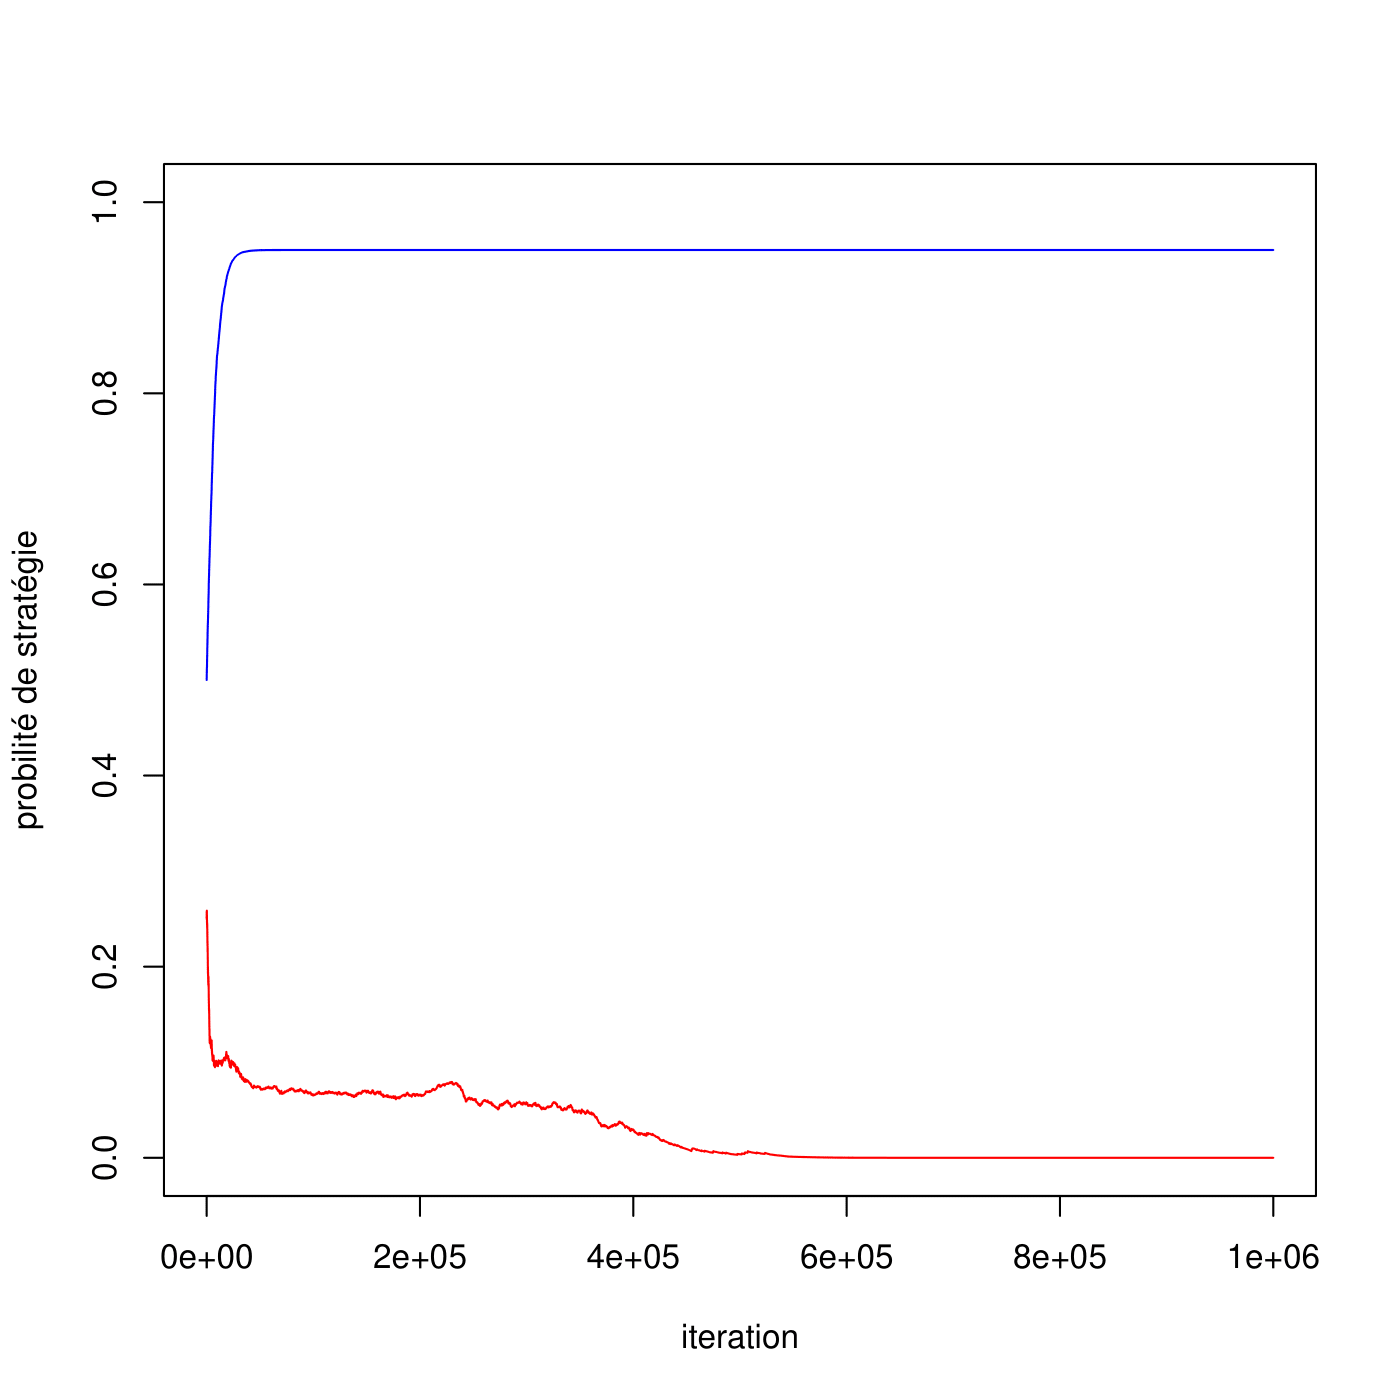
\includegraphics[width =\textwidth]{Images/Courbes/LRI/Relance1.png}
       
    
        \end{column}
       
        \begin{column}{0.5 \textwidth}
         \begin{small}
          \hspace{-0.24 cm} Probabilité qu'\textcolor{red}{Alice} relance de 2\\ Probabilité que \textcolor{blue}{Bob} suive\\
          \end{small}
        \centering
            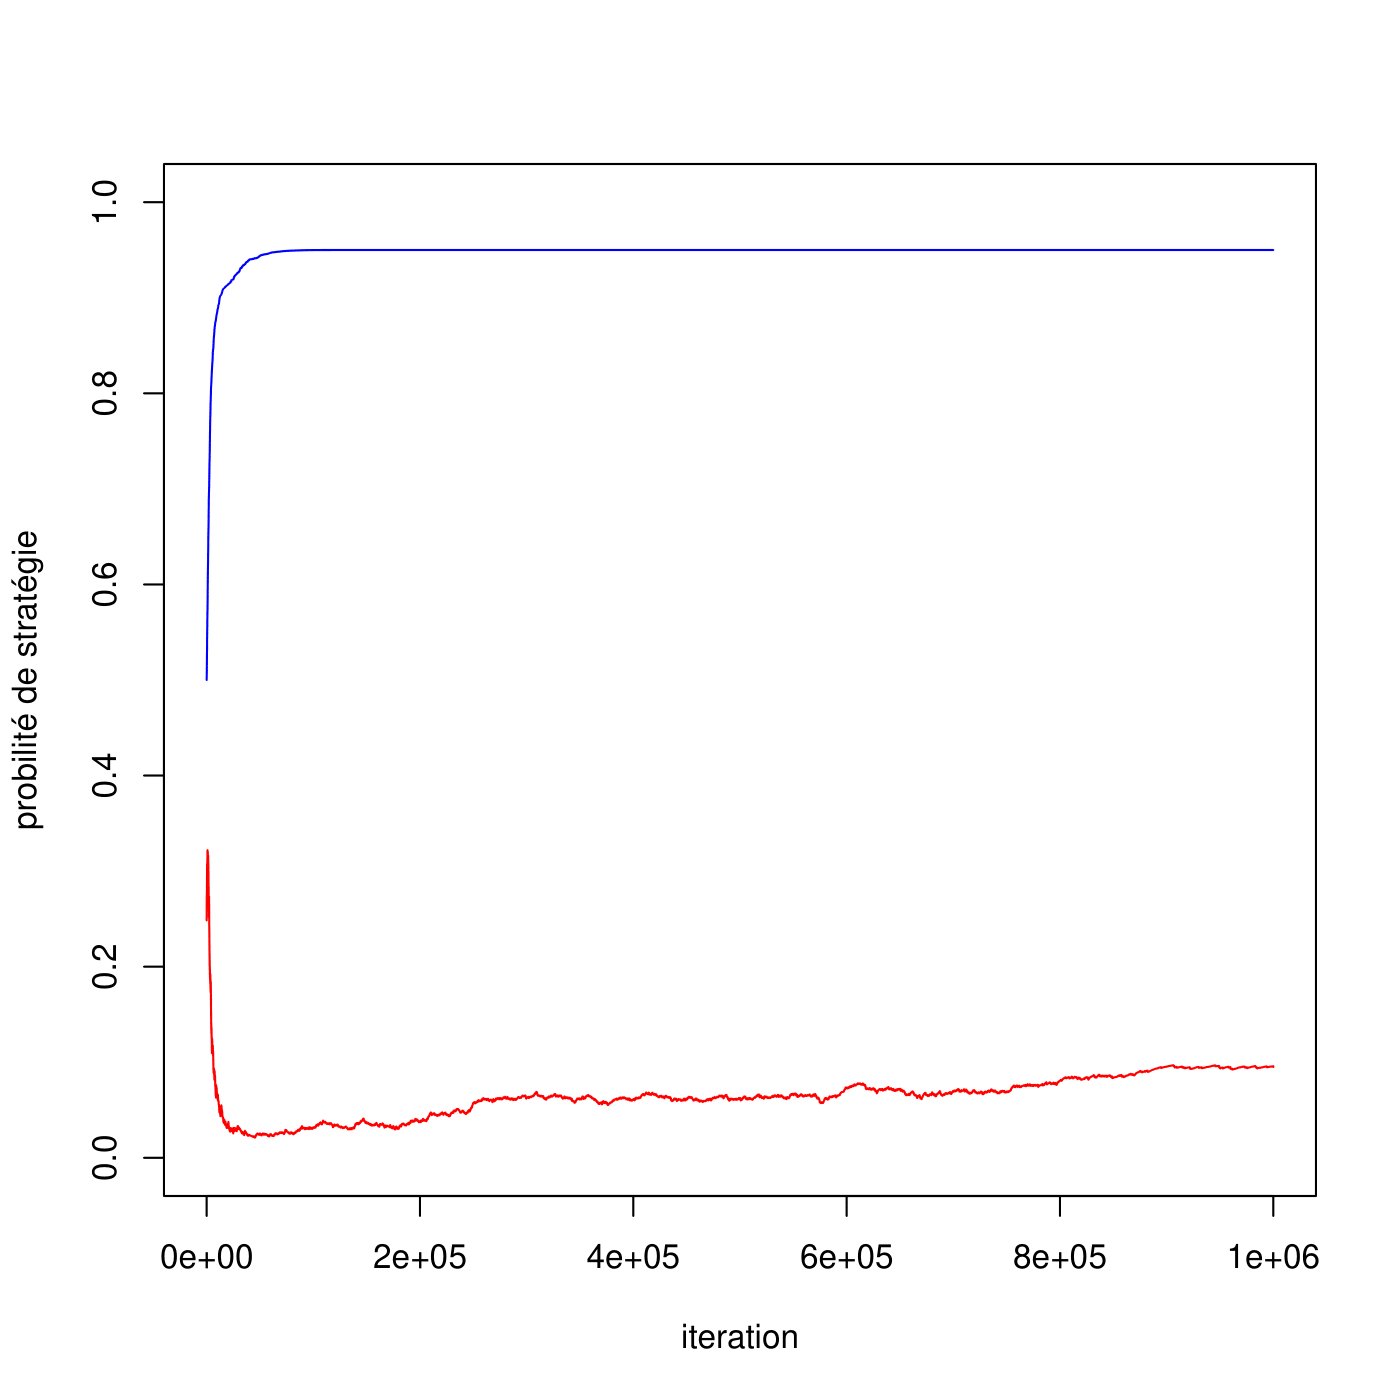
\includegraphics[width =\textwidth]{Images/Courbes/LRI/Relance2.png}
       
    \end{column}
    \end{columns}
\end{frame}

\begin{frame}{Étude de courbes}
Courbes des gains de \textcolor{blue}{Bob} et d\textcolor{red}{Alice} .
\centering
    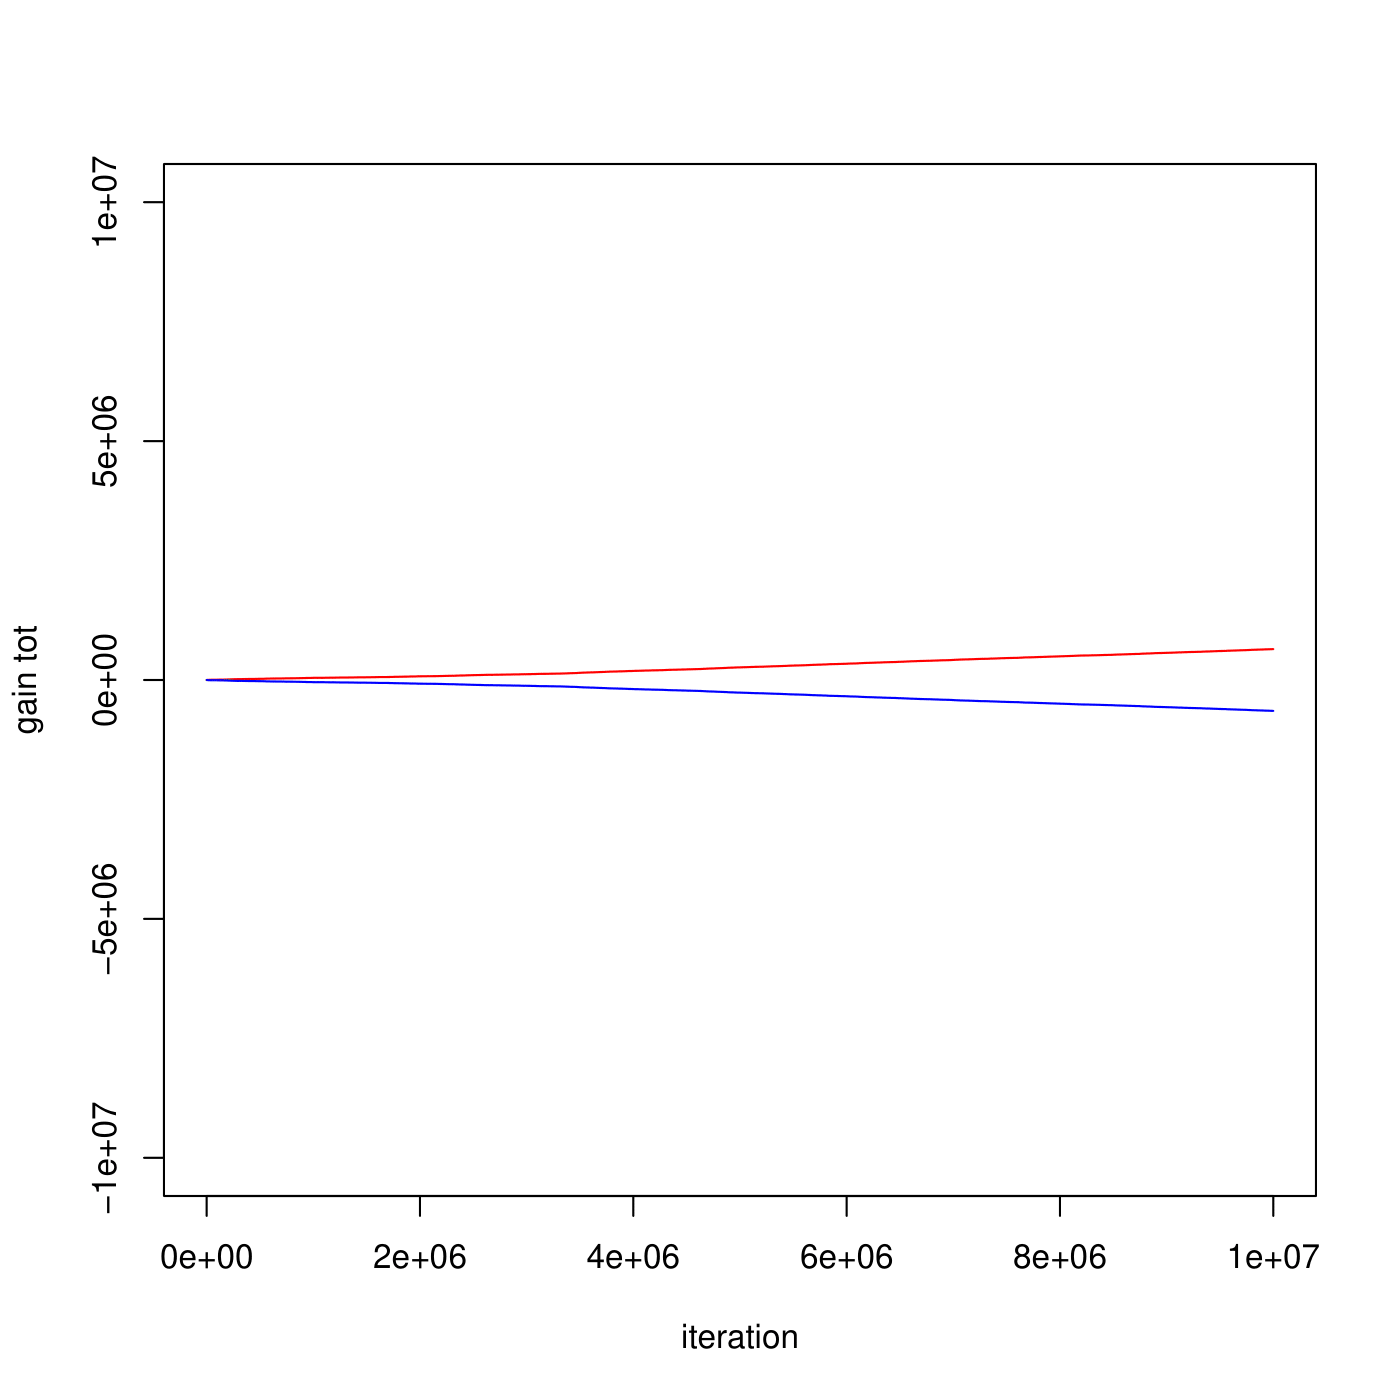
\includegraphics[width =1 \textwidth, height = 0.8 \textheight]{Images/Courbes/LRI/Gain.png}
\end{frame}


\include{Diapos/AppLRI}
\section{Linear Reward Penalty}
\subsection{Principe}

\begin{frame}{Principe}
\begin{itemize}
    \item Repose sur un \textbf{principe de récompense} lors d'une action positive.
    \item \textbf{Pénalise} les mauvaises actions.\\~\
    \item On obtient un \textbf{vecteur stochastique de stratégies} pour chaque carte et joueurs qui \textbf{se met à jour lors d'un gain ou d'une perte}.
\end{itemize}
\end{frame}

\begin{frame}{Mise à jour des stratégies des joueurs}
    \begin{block}{Règle de Mise à jour}
    \fontsize{8pt}{15pt}
    $q_{i,s}(t+1)=\left\{
    \begin{array}{ll}
        q_{i,s}(t)+b*U_{t}*(1-q_{i,s}(t))-\beta*q_{i,s}(t)* (1-U_{t}) & \mbox{Si } s=s_i(t) \\
         q_{i,s}(t)-b*U_{t}*q_{i,s}(t)+\beta*((k-1)^{-1}- q_{i,s}(t))*(1-U_{t}) & \mbox{Si } s\neq s_i(t)
    \end{array}
\right.$
    \end{block}
    
    \begin{exampleblock}{Variables et constantes}
    \begin{description}
    
    \item[b] : paramètre d'apprentissage tq $b \in [0,1]$ et $b\leq \frac{1}{U_{max}}$.
    \item[$\beta$] : paramètre d'apprentissage tq $\beta \in [0,1]$
    \item[k] : nombre total des actions.
    \item[$q_{i,s}(t)$] : probabilité que le joueur i joue la stratégie s à l'étape t.
    \item[$U_t$] : fonction d'utilité. %$U_t = \frac{Gain}{GainMax} =  \frac{Gain}{5}$
    
    \end{description}
    \end{exampleblock}
    
\end{frame}

\begin{frame}{Mise à jour des stratégies des joueurs}
    \begin{block}{Règle de Mise à jour}
    \fontsize{8pt}{15pt}
    $q_{i,s}(t+1)=\left\{
    \begin{array}{ll}
        q_{i,s}(t)+b*U_{t}*(1-q_{i,s}(t))-\beta*q_{i,s}(t)* (1-U_{t}) & \mbox{Si } s=s_i(t) \\
         q_{i,s}(t)-b*U_{t}*q_{i,s}(t)+\beta*((k-1)^{-1}- q_{i,s}(t))*(1-U_{t}) & \mbox{Si } s\neq s_i(t)
    \end{array}
\right.$
    \end{block}
    
    \begin{exampleblock}{Décision du choix des règles}
    
    $\left\{\begin{array}{ll}
    Linear\quad Reward\quad Penalty & \mbox{Si } b = \beta  \\
    Linear\quad Reward\quad Inaction & \mbox{Si } \beta = 0 \\
    Linear\quad Reward\quad \varepsilon-Penalty & \mbox{Si } b >> \beta 
    \end{array} 
    \right.$
    
    \end{exampleblock}
    
\end{frame}

\subsection{Application}

\begin{frame}{Etude de courbes}
    \begin{columns}
        \begin{column}{0.5 \textwidth}
        \begin{small}
        \hspace{-0.24 cm} Probabilité qu'\textcolor{red}{Alice} relance de 4 \\  Probabilité que \textcolor{blue}{Bob} suive\\
        \end{small}
        \centering
            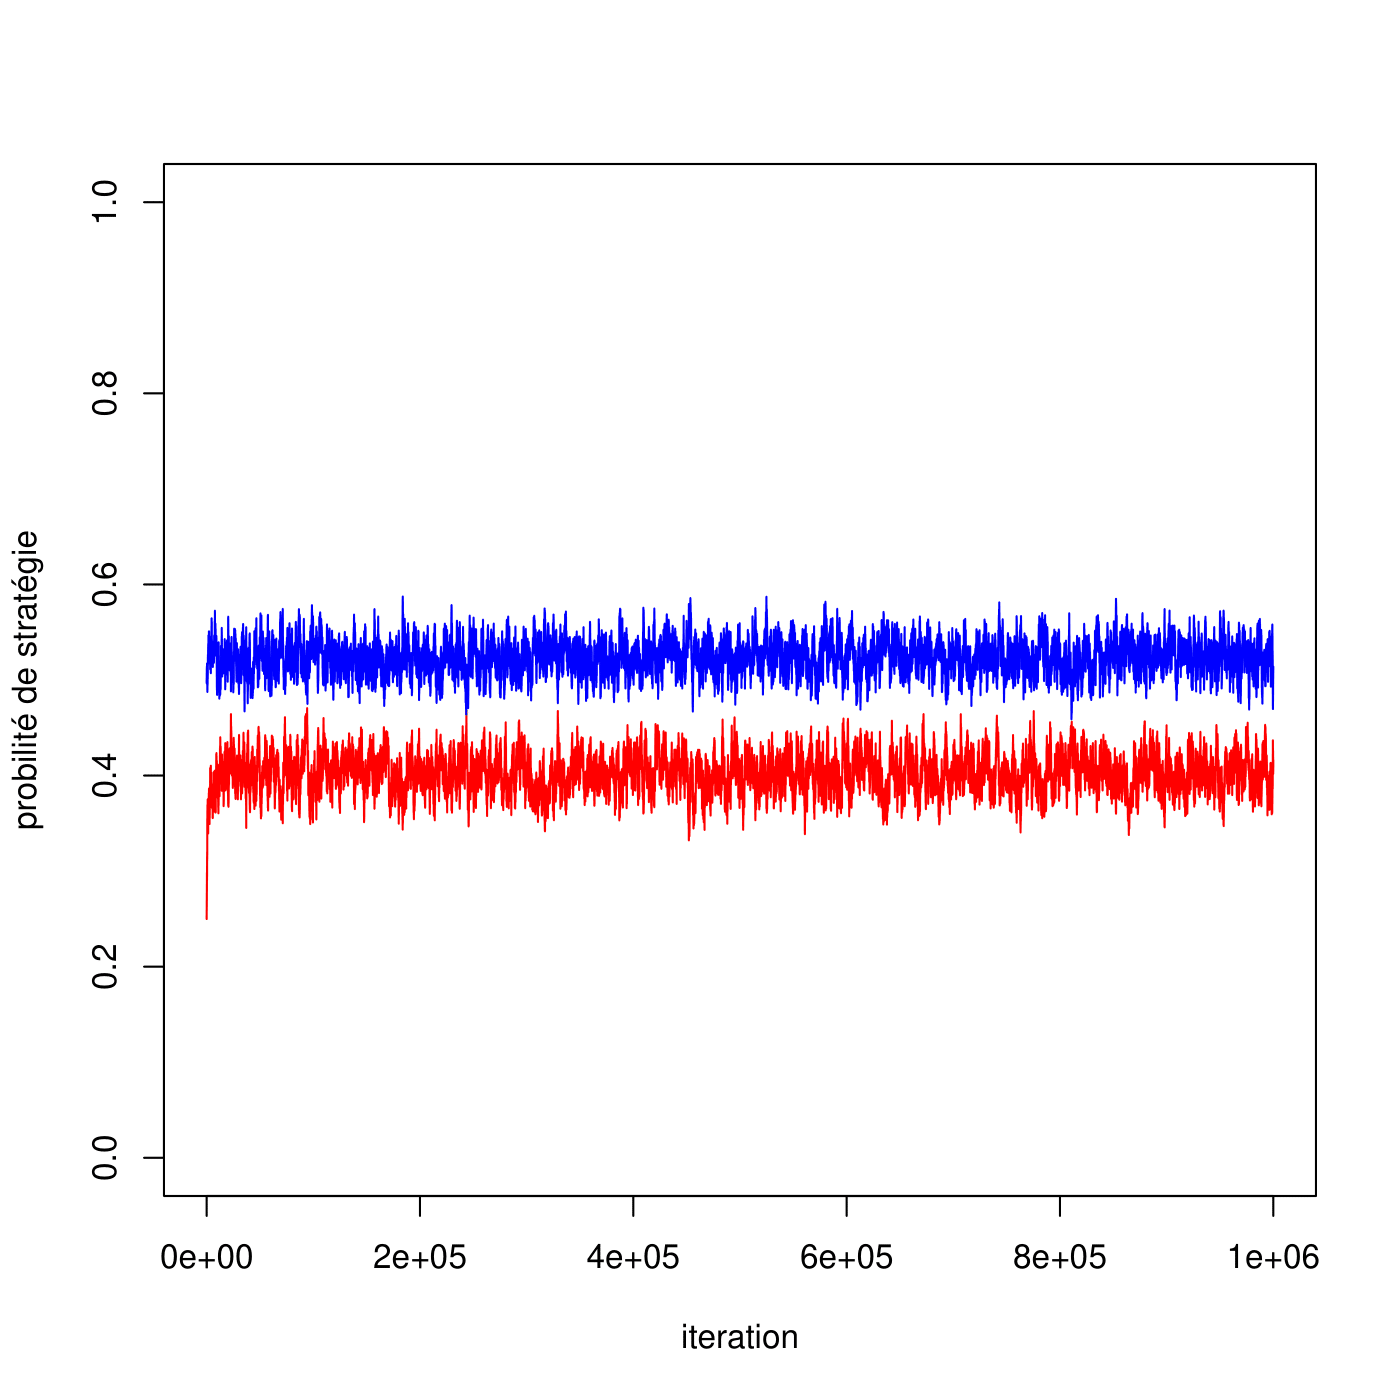
\includegraphics[width =\textwidth]{Images/Courbes/lrp-1.png}
       
    
        \end{column}
       
        \begin{column}{0.5 \textwidth}
         \begin{small}
          \hspace{-0.24 cm} Gain total d'\textcolor{red}{Alice} et de \textcolor{blue}{Bob} 
          \end{small}
        \centering
            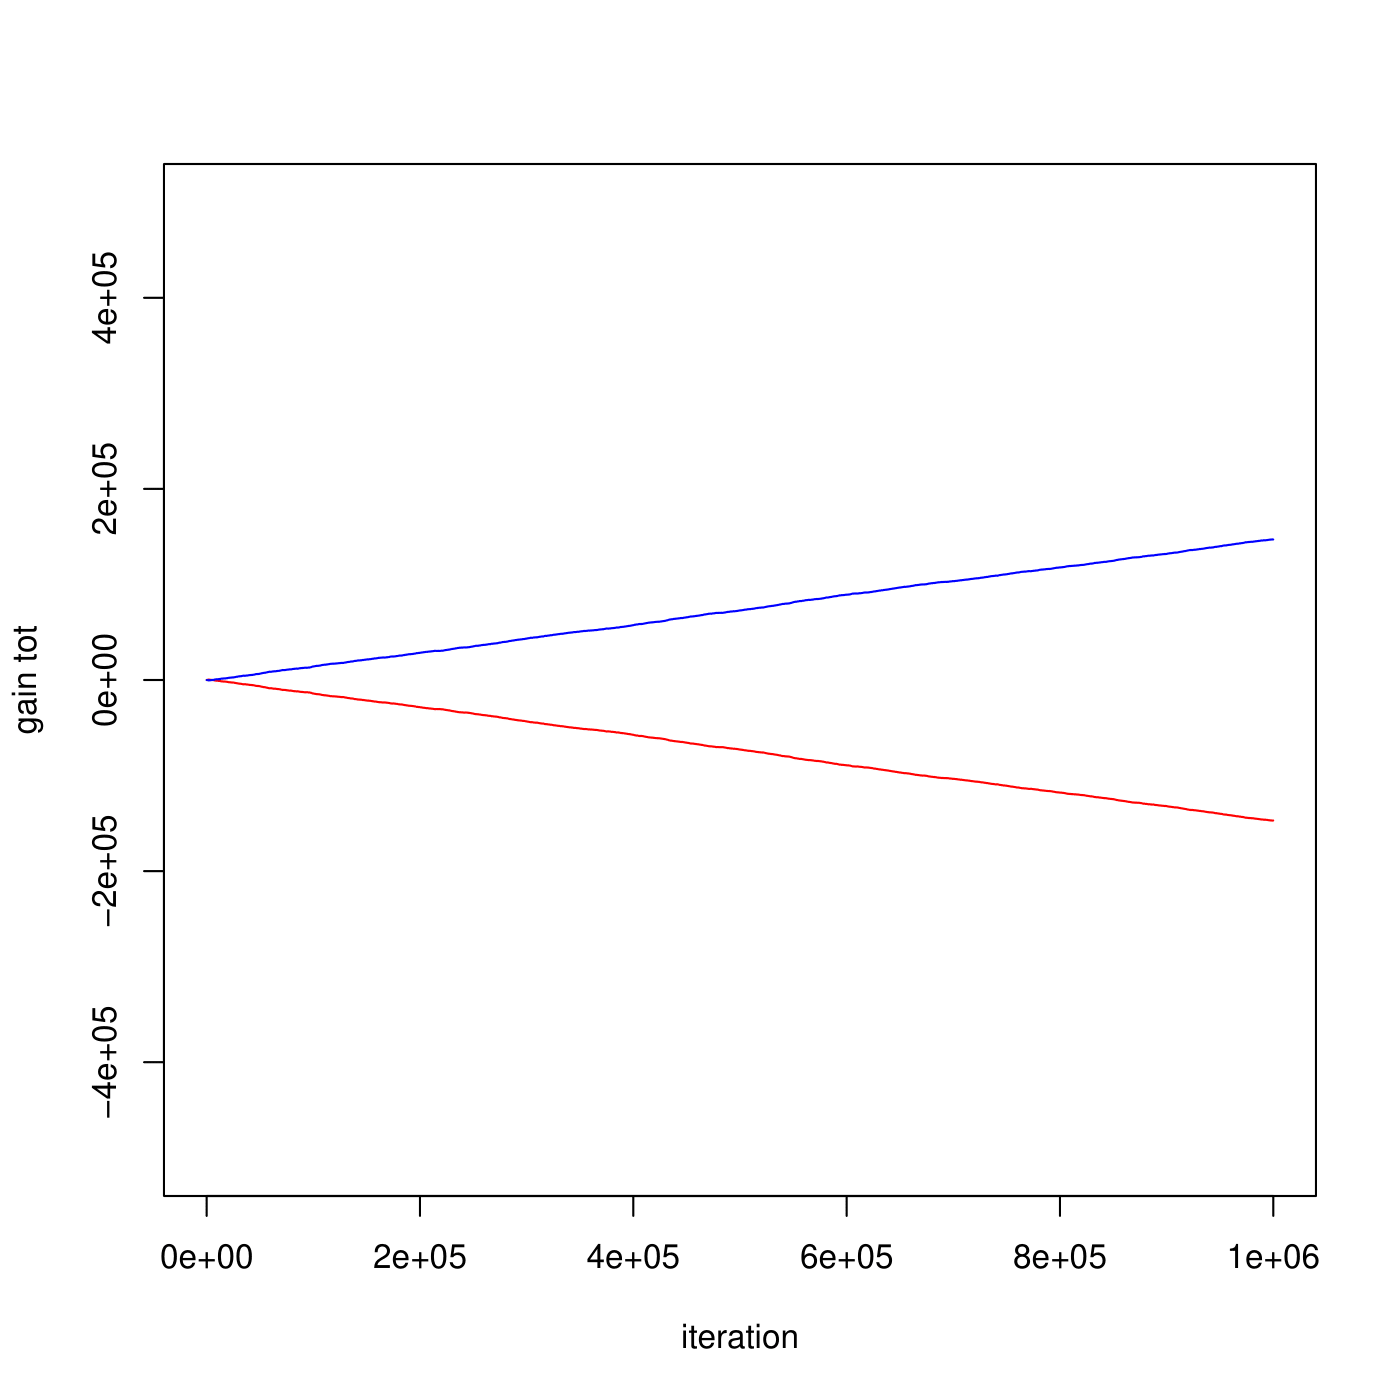
\includegraphics[width =\textwidth]{Images/Courbes/lrp-2.png}
       \end{column}
        \end{columns}



    
\end{frame}
\section{Conclusion}
\begin{frame}{Conclusion}
\begin{itemize}
    \item LRI est peu efficace sur des jeux avec perte.
    \item LRP est donc plus intéressant sur ce jeu.
\end{itemize}
\end{frame}

\end{document}
